\documentclass[10pt,a4paper]{article}

%------------------------------------------------------------------------------
%	REQUIRED PACKAGES AND  CONFIGURATIONS
%------------------------------------------------------------------------------

% PACKAGES FOR TITLES
\usepackage{titlesec}
\usepackage{color}

% PACKAGES FOR LANGUAGE AND FONT
\usepackage[utf8]{inputenc}
\usepackage[english]{babel}
\usepackage[T1]{fontenc} % Font encoding
\usepackage{kpfonts}
\tolerance=1
\emergencystretch=\maxdimen
\hyphenpenalty=10000
\hbadness=10000
\vfuzz=30pt

% PACKAGES FOR IMAGES
\usepackage{graphicx}
\graphicspath{{Images/}} % Path for images' folder
\usepackage{eso-pic} % For the background picture on the title page
\usepackage{subfig} % Numbered and caption subfigures using \subfloat
\usepackage{caption} % Coloured captions
\usepackage{transparent}
\usepackage{wrapfig}

% STANDARD MATH PACKAGES
\usepackage{amsmath}
\usepackage{amsthm}
\usepackage{bm}
\usepackage[overload]{empheq}  % For braced-style systems of equations
\usepackage{matlab-prettifier}
\usepackage{gensymb}

% PACKAGES FOR TABLES
\usepackage{tabularx}
\usepackage{longtable} % tables that can span several pages
\usepackage{colortbl}
\usepackage{xltabular}
\usepackage{makecell}

% PACKAGES FOR ALGORITHMS (PSEUDO-CODE)
\usepackage{algorithm}
\usepackage{algorithmic}

% PACKAGES FOR REFERENCES & BIBLIOGRAPHY
\usepackage{hyperref} % Adds clickable links at references
\hypersetup{
	colorlinks=true,
	linkcolor=bluePoli,
	anchorcolor=black,
	citecolor=bluePoli,
	filecolor=black,
	menucolor=black,
	runcolor=black,
	urlcolor=black,
}
\usepackage{cleveref}
\usepackage[super,square,numbers,sort&compress]{natbib}
\bibliographystyle{unsrt}
\usepackage{tocbibind}

% PACKAGES FOR THE APPENDIX
\usepackage[page]{appendix}
\renewcommand{\appendixpagename}{\Large\color{bluePoli}Appendice}

% PACKAGES FOR ITEMIZE & ENUMERATES 
\usepackage{enumitem}

% OTHER PACKAGES
\usepackage{amsthm,thmtools,xcolor} % Coloured "Theorem"
\usepackage{comment} % Comment part of code
\usepackage{fancyhdr} % Fancy headers and footers
\usepackage{lipsum} % Insert dummy text
\usepackage{tcolorbox} % Create coloured boxes (e.g. the one for the key-words)
\usepackage{stfloats} % Correct position of the tables
\usepackage{cuted}
\usepackage{multicol}

%-------------------------------------------------------------------------
%	NEW COMMANDS DEFINED
%-------------------------------------------------------------------------

% EXAMPLES OF NEW COMMANDS -> here you see how to define new commands
\newcommand{\bea}{\begin{eqnarray}} % Shortcut for equation arrays
\newcommand{\eea}{\end{eqnarray}}
\newcommand{\e}[1]{\times 10^{#1}}  % Powers of 10 notation
\newcommand{\mathbbm}[1]{\text{\usefont{U}{bbm}{m}{n}#1}} % From mathbbm.sty
\newcommand{\pdev}[2]{\frac{\partial#1}{\partial#2}}
% NB: you can also override some existing commands with the keyword \renewcommand

%----------------------------------------------------------------------------
%	ADD YOUR PACKAGES (be careful of package interaction)
%----------------------------------------------------------------------------


%----------------------------------------------------------------------------
%	ADD YOUR DEFINITIONS AND COMMANDS (be careful of existing commands)
%----------------------------------------------------------------------------

\DeclareMathOperator{\atantwo}{atan2}

\newcommand{\twofig}[6]{
\begin{figure}[H]
	\begin{minipage}{0.48\linewidth}
		\centering
		\includegraphics[width=\linewidth]{#1}
		\caption{#2}
		\label{fig:#3}
	\end{minipage}\hfill
	\begin{minipage}{0.48\linewidth}
		\centering
		\includegraphics[width=\linewidth]{#4}
		\caption{#5}
		\label{fig:#6}
	\end{minipage}
\end{figure}
}

\newcommand{\twofigII}[7]{
\begin{figure}[H]
	\begin{minipage}{0.48\linewidth}
		\centering
		\includegraphics[width=#7\linewidth]{#1}
		\caption{#2}
		\label{fig:#3}
	\end{minipage}\hfill
	\begin{minipage}{0.48\linewidth}
		\centering
		\includegraphics[width=#7\linewidth]{#4}
		\caption{#5}
		\label{fig:#6}
	\end{minipage}
\end{figure}
}

\newcommand{\cfig}[4]{
\begin{figure}[H]
	\centering
	\includegraphics[width=#4\linewidth]{#1}
	\caption{#2}
	\label{fig:#3}
\end{figure}
}

\newcommand{\rfig}[4]{
\begin{wrapfigure}{r}{#4\linewidth}
	\centering
	\includegraphics[width=\linewidth]{#1}
	\caption{#2}
	\label{fig:#3}
	\vspace*{-13pt}
\end{wrapfigure}
}

\newcommand{\lfig}[4]{
\begin{wrapfigure}{l}{#4\linewidth}
	\centering
	\includegraphics[width=\linewidth]{#1}
	\caption{#2}
	\label{fig:#3}
	\vspace*{-13pt}
\end{wrapfigure}
}


% Do not change Configuration_files/config.tex file unless you really know what you are doing. 
% This file ends the configuration procedures (e.g. customizing commands, definition of new commands)
% Set the geometric layout of the document
\usepackage{geometry}
\geometry{
  top=2.5cm,
  left = 1.5cm,
  right = 1.5cm,
  bottom=1.5cm,
  headheight= 2.2cm,
  headsep= 0cm,
}
\raggedbottom 

% Create color bluePoli (-> manuale grafica coordinata:  https://www.polimi.it/fileadmin/user_upload/il_Politecnico/grafica-coordinata/2015_05_11_46xy_manuale_grafica_coordinata.pdf)
\definecolor{bluePoli}{cmyk}{0.4,0.1,0,0.4}

% Custom theorem environments
\declaretheoremstyle[
  headfont=\color{bluePoli}\normalfont\bfseries,
  bodyfont=\color{black}\normalfont\itshape,
]{colored}

\captionsetup[figure]{labelfont={color=bluePoli}} % Set colour of the captions
\captionsetup[table]{labelfont={color=bluePoli}} % Set colour of the captions
%\captionsetup[algorithm]{labelfont={color=bluePoli}} % Set colour of the captions

\theoremstyle{colored}
\newtheorem{theorem}{Theorem}[section]
\newtheorem{proposition}{Proposition}[section]

% Enhances the features of the standard "table" and "tabular" environments.
\newcommand\T{\rule{0pt}{2.6ex}}
\newcommand\B{\rule[-1.2ex]{0pt}{0pt}}

% Algorithm description
\newcounter{algsubstate}
\renewcommand{\thealgsubstate}{\alph{algsubstate}}
\newenvironment{algsubstates}{
    \setcounter{algsubstate}{0}%
    \renewcommand{\STATE}{%
    \stepcounter{algsubstate}%
    \Statex {\small\thealgsubstate:}\space}
    }{}
    
% Custom theorem environment
\newcolumntype{L}[1]{>{\raggedright\let\newline\\\arraybackslash\hspace{0pt}}m{#1}}
\newcolumntype{C}[1]{>{\centering\let\newline\\\arraybackslash\hspace{0pt}}m{#1}}
\newcolumntype{R}[1]{>{\raggedleft\let\newline\\\arraybackslash\hspace{0pt}}m{#1}}

% Custom itemize environment
\setlist[itemize,1]{label=$\bullet$}
\setlist[itemize,2]{label=$\circ$}
\setlist[itemize,3]{label=$-$}
\setlist{nosep}

% Create command for background pic
\newcommand\BackgroundPic{% Adding background picture
	\put(230,358){
		\parbox[b][\paperheight]{\paperwidth}{%
			\vfill
			\centering
			\transparent{0.4}
			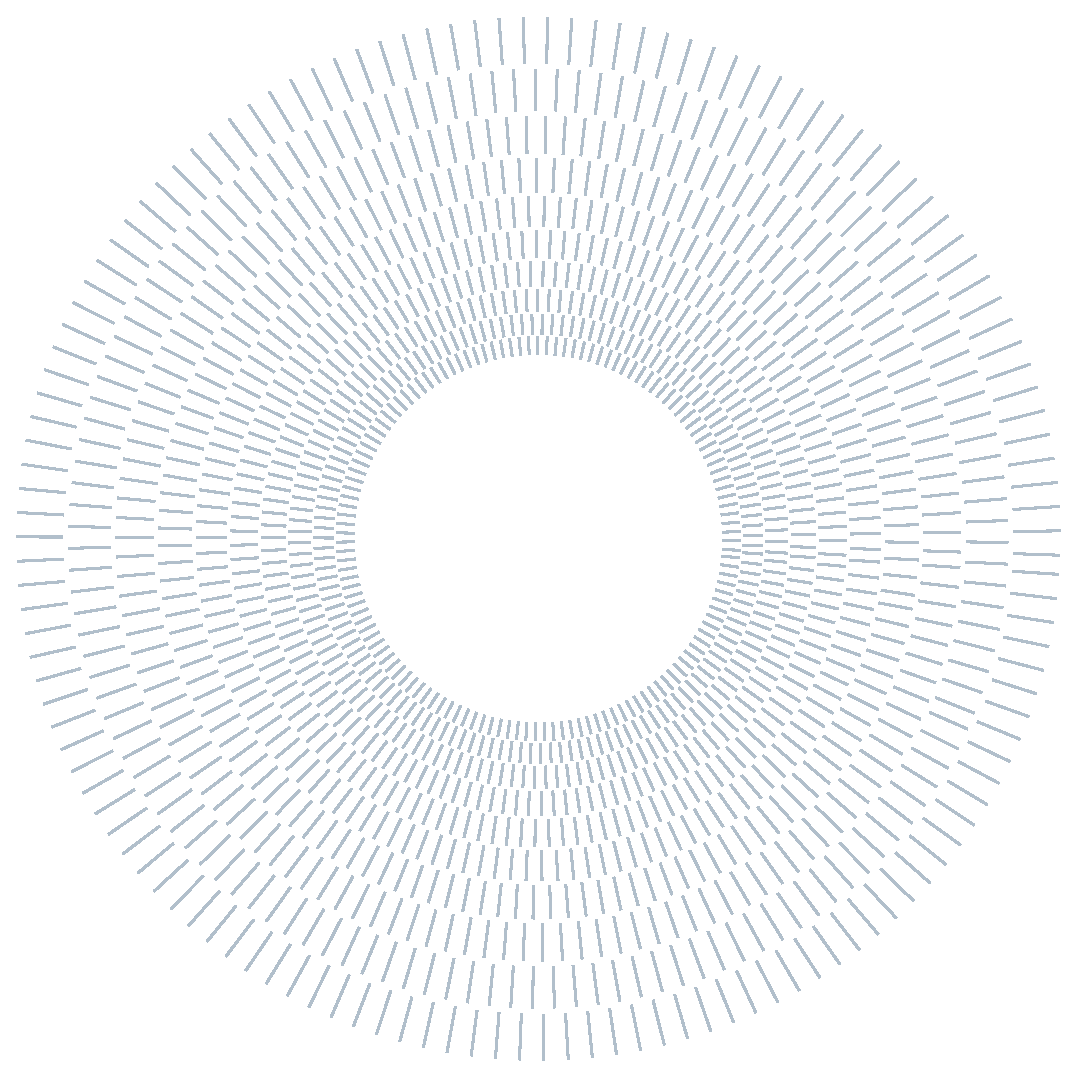
\includegraphics[width=0.5\paperwidth]{raggiera_polimi.eps}%
			\vfill
}}}

% Set indentation
\setlength\parindent{0pt}

% Set abstract
\renewenvironment{abstract}{\section*{\abstractname}}{}

% Custom title commands
\titleformat{\section}
{\color{bluePoli}\normalfont\Large\bfseries}
{\color{bluePoli}\thesection.}{1em}{}
\titlespacing*{\section}
{0pt}{2ex}{1ex}

\titleformat{\subsection}
{\color{bluePoli}\normalfont\large\bfseries}
{\color{bluePoli}\thesubsection.}{1em}{}
\titlespacing*{\subsection}
{0pt}{2ex}{1ex}

% Custom headers and footers
\pagestyle{fancy}
\fancyhf{}
      
\fancyfoot{}
\fancyfoot[C]{\thepage} % page
\renewcommand{\headrulewidth}{0mm} % headrule width
\renewcommand{\footrulewidth}{0mm} % footrule width

\makeatletter
\patchcmd{\headrule}{\hrule}{\color{black}\hrule}{}{} % headrule
\patchcmd{\footrule}{\hrule}{\color{black}\hrule}{}{} % footrule
\makeatother

% -> Create the header
\chead[C]{
\centering
\begin{tcolorbox}[arc=0pt, boxrule=0pt, colback=bluePoli!60, width=\textwidth, colupper=white]
    \textbf{Simulation of a LEO orbiting microsat on Simulink} \hfill \textbf{\author}  
\end{tcolorbox}
}

%-----------------------------------------------------------------------------

% Insert here the info that will be displayed into your Title page 
% -> title of your work
\renewcommand{\title}{Simulation of a LEO orbiting microsat on Simulink}

% -> author name and surname
\newcommand{\authors}{
\begin{tabular}{rll}
    10723712	&	Marcello Pareschi	&	(BSc Aerospace Engineering - Politecnico di Milano)\\
    10836125	&	Daniele Paternoster	&	(BSc Aerospace Engineering - Politecnico di Milano)\\
    10711624	&	Alex Cristian Turcu	&	(BSc Aerospace Engineering - Politecnico di Milano)\\
    10884250	&	Tamim Harun	Or		&	(BCs Aerospace Engineering - International Islamic University Malaysia)
\end{tabular}
}

% -> MSc course
\newcommand{\course}{Space Engineering}

% -> advisor name and surname
\newcommand{\professor}{Franco Bernelli Zazzera}

% IF AND ONLY IF you need to modify the co-supervisors you also have to modify the file Configuration_files/title_page.tex (ONLY where it is marked)
%\newcommand{\firstcoadvisor}{Name Surname} % insert if any otherwise comment
%\newcommand{\secondcoadvisor}{Name Surname} % insert if any otherwise comment

% -> academic year
\newcommand{\YEAR}{2023-2024}

\begin{document}
\pagenumbering{Roman}

%-----------------------------------------------------------------------------
% TITLE PAGE
%-----------------------------------------------------------------------------

% Do not change Configuration_files/TitlePage.tex (Modify it IF AND ONLY IF you need to add or delete the Co-advisors)
% This file creates the Title Page of the document
% DO NOT REMOVE SPACES BETWEEN LINES!

\let\temp\newpage
\let\newpage\relax
\begin{titlepage}

\AddToShipoutPicture*{\BackgroundPic}

\hspace{-0.6cm}
\includegraphics[width=0.6\textwidth]{logo_polimi_ing_indinf.eps}

\vspace{-0.2cm}
\Large{\textbf{\color{bluePoli}{\title}}}\\
\hspace*{\fill}

\vspace{-0.2cm}
\fontsize{0.3cm}{0.5cm}\selectfont \bfseries \textsc{\color{bluePoli} MSc in \course}\\
\hspace*{\fill}

\vspace{-0.2cm}
\fontsize{0.3cm}{0.5cm} \selectfont \bfseries Authors:\par
\vspace{0.2cm} \hspace{0.3cm} \textsc{\textbf{\authors}}\\
\hspace*{\fill}

\fontsize{0.3cm}{0.5cm}\selectfont \bfseries Professor: \textsc{\textbf{\professor}}\\
\hspace*{\fill}

% if only ONE co-advisor is present:
%\vspace{-0.4cm}
%\fontsize{0.3cm}{0.5cm}\selectfont \bfseries Co-advisor: %\textsc{\textbf{\firstcoadvisor}}\\
% if more than one co-advisors are present:
%\vspace{-0.4cm}
%\fontsize{0.3cm}{0.5cm}\selectfont \bfseries Co-advisors: \textsc{\textbf{\firstcoadvisor}}\textsc{\textbf{\secondcoadvisor}}\\

\vspace{-0.4cm}
\fontsize{0.3cm}{0.5cm}\selectfont \bfseries Academic year: \textsc{\textbf{\YEAR}}

\small \normalfont

\vspace{11pt}

\centerline{\rule{1.0\textwidth}{0.4pt}}

\vspace{15pt}

\end{titlepage}
\let\newpage\temp

\thispagestyle{plain} % In order to not show the header in the first page

\vspace{15mm}
\begin{abstract}
\addcontentsline{toc}{section}{Abstract}
\vspace*{5mm}

The following report discusses the attitude dynamics and control of a microsatellite in Sun-synchronous low-Earth orbit. The mission of the satellite is to point the Earth, due to the payload requirement. The simulation was carried out in Simulink environment. The rotational dynamics was modeled through the Euler equations, the kinematics was parametrized through two sets of Euler angles (312 - 313). The environment disturbances that was accounted for were the magnetic field interaction and gravity gradient torque. They were considered the most relevant after a general analysis of all the four main disturbances (SRP, air drag torque, magentic torque, gravity gradient torque). The orbital motion was modeled as a restricted two body problem. 

The on-board sensors were a horizon sensor, a magnetometer and a sun sensor. They were all modeled in Simulink, taking as reference real sensors. The actuators installed on the satellite were a magnetorquer and two reaction wheels, modeled referring to real actuators. 

The control logic implemented on-board considers two algorithms. The first deals with the de-tumbling of the spacecraft using the B-dot control, until a certain condition on the value of the derivative of B is satisfied. The second contemplates the slew and tracking manoeuvre togheter. This last phase is performed through an extension of the PD controller for non-linear dynamics. 


\end{abstract}
\clearpage


%-----------------------------------------------------------------------------

%-----------------------------------------------------------------------------
% INDEX
%-----------------------------------------------------------------------------

{\hypersetup{linkcolor=black}\tableofcontents}

\clearpage

%-----------------------------------------------------------------------------

%{\hypersetup{linkcolor=black}\listoftables}


%-----------------------------------------------------------------------------

%{\hypersetup{linkcolor=black}\listoffigures}

%\clearpage

%-----------------------------------------------------------------------------

\section{Symbols}
\label{sec:symbols}
\setcounter{subsection}{2}
\newsavebox\ltmcbox
\renewcommand{\arraystretch}{1.2}
\renewcommand\tabularxcolumn[1]{m{#1}}

\begin{multicols}{2}
	\raggedcolumns

	\subsection{Framework analysis}
	\vspace{-10pt}
	\small
	\setbox\ltmcbox\vbox{
	\makeatletter\col@number\@ne
	\begin{xltabular}{\linewidth}{cc>{\raggedright\arraybackslash}X}
		$\bm{I}$ & $[kg/m^2]$ & inertia matrix \\
		$a$ & $[km]$ & semi-major axis \\
		$e$ & $[-]$ & eccentricty \\
		$i$ & $[deg]$ & inclination \\
		$\omega$ & $[deg]$ & pericentre anomaly \\
		$\Omega$ & $[deg]$ & RAAN \\
		$\theta$ & $[rad]$ & true anomaly \\
		$n$ & $[rad/s]$ & mean anomaly \\
		$\mathcal{P}$ & $[-]$ & perifocal frame \\
		$\mathcal{N}$ & $[-]$ & inertial frame \\
		$\bm{A_{PN}}$ & $[-]$ & rotation matrix from intertial to perifocal frame\\
		$\bm{r_p}$ & $[km]$ & S/C position in $\mathcal{P}$ frame \\
		$\bm{r_p}$ & $[km]$ & S/C position in $\mathcal{N}$ frame 
	\end{xltabular}
	\unskip
	\unpenalty
	\unpenalty}
	\unvbox\ltmcbox

	\subsection{Dynamics}
	\vspace{-10pt}
	\small
	\setbox\ltmcbox\vbox{
	\makeatletter\col@number\@ne
	\begin{xltabular}{\linewidth}{cc>{\raggedright\arraybackslash}X}
		$\mathcal{B}$ & $[-]$ & body frame \\
		$\bm{x_b}$ & $[-]$ & x direction of the $\mathcal{B}$ frame \\
		$\bm{y_b}$ & $[-]$ & y direction of the $\mathcal{B}$ frame \\
		$\bm{z_b}$ & $[-]$ & z direction of the $\mathcal{B}$ frame \\
		$\bm{\omega}$ & $[rad/s]$ & angular velocity in $\mathcal{B}$ frame \\
		$\bm{\dot{\omega}}$ & $[rad/s]$ & angular velocity rate in $\mathcal{B}$ frame \\
		$\bm{M_d}$ & $[Nm]$ & disturbances torque \\
		$\bm{M_c}$ & $[Nm]$ & control torque 
	\end{xltabular}
	\unskip
	\unpenalty
	\unpenalty}
	\unvbox\ltmcbox

	\subsection{Kinematics}
	\vspace{-10pt}
	\small
	\setbox\ltmcbox\vbox{
	\makeatletter\col@number\@ne
	\begin{xltabular}{\linewidth}{cc>{\raggedright\arraybackslash}X}
		$\bm{s}$ & $[rad]$ & set of Euler angles \\
		$\bm{\dot{s}}$ & $[rad/s]$ & set of Euler angle's rates \\
		$312$ & $[-]$ & sequence of axis' rotation \\
		$313$ & $[-]$ & sequence of axis' rotation \\
		$\phi$ & $[rad]$ & first rotation's angle \\
		$\theta$ & $[rad]$ & second rotation's angle \\
		$\psi$ & $[rad]$ & third rotation's angle \\
		$\bm{A_{BN}}$ & $[Nm]$ & attitude matrix \\
		$tol$ & $[-]$ & tolerance value for singularity check 
	\end{xltabular}
	\unskip
	\unpenalty
	\unpenalty}
	\unvbox\ltmcbox

	\subsection{Disturbances analysis}
	\vspace{-10pt}
	\small
	\setbox\ltmcbox\vbox{
	\makeatletter\col@number\@ne
	\begin{xltabular}{\linewidth}{cc>{\raggedright\arraybackslash}X}
		$\bm{M}$ & $[Nm]$ & disturbance torque \\
		$\bm{D}$ & $[Am^{2}]$ & magnetic dipole from coils or parasitic currents \\
		$\bm{B}$ & $[T]$ & magnetic field \\
		$V$      & $[Tm]$ & magnetic field scalar potential \\
		$ECEF$   & [-] & Earth Centered Earth Fixed frame \\
		$r$ & $[m]$ & radial distance from Earth's centre to S/C position (ECEF) \\
		$\theta$ & $[rad]$ & longitude (ECEF) \\
		$\phi$ & $[rad]$ & co-latitude (ECEF) \\
        $P^{n,m} (\cos \theta)$ & $[-]$ & Gauss normalized associated Legendre functions \\
		$g^{n,m} (t)$ & $[nT]$ & Schmidt semi-normalized spherical harmonic coefficients \\
        $h^{n,m} (t)$ & $[nT]$ & Schmidt semi-normalized spherical harmonic coefficients \\
		$F_i$ & $[N]$ & disturbance force acting on i-th panel \\
		$P$ & $[Pa]$ & Sun's pressure of radiation \\
		$A_i$ & $[Pa]$ & area of i-th panel \\
		$\bm{\hat{S}_B}$ & $[-]$ & Sun's direction in $\mathcal{B}$ frame \\
		$\bm{\hat{N}_{B,i}}$ & $[-]$ &  i-th panel's normal direction in $\mathcal{B}$ frame \\
		$\rho_s$ & $[-]$ & coefficient of specular reflection \\
		$\rho_a$ & $[-]$ & coefficient of absorption \\
		$\rho_d$ & $[-]$ & coefficient of diffusion \\
		$\epsilon$ & $[deg]$ & obliquity of Earth \\
		$C_D$ & $[-]$ & coefficient of drag \\
		$\bm{r_i}$ & $[m]$ & position of centre of action of the force \\
		$\bm{v_{B,i}}$ & $[m/s]$ & relative velocity in $\mathcal{B}$ frame of the i-th panel \\
		$\bm{\hat{v}_{B,i}}$ & $[s^{-1}]$ & direction of relative velocity in $\mathcal{B}$ frame of the i-th panel \\
		$\rho$ & $[kg/m^3]$ & denisty of air \\
		$\rho_0$ & $[kg/m^3]$ & reference denisty of air from US Standard Atmosphere model (1976)\\
		$h_0$ & $[km]$ & reference heigh from US Standard Atmosphere model (1976)\\
		$H$ & $[km]$ & scaling height from US Standard Atmosphere model (1976)\\
		$G$ & $[m^3 kg^{-1} s^{-2}]$ & universal gravitational constant \\
		$m_t$ & $[kg]$ & mass of Earth \\
		$c_i$ & $[-]$ & director cosines of the radial direction in the $\mathcal{B}$ frame \\
	\end{xltabular}
	\unskip
	\unpenalty
	\unpenalty}
	\unvbox\ltmcbox

	\subsection{Sensors}
	\vspace{-10pt}
	\small
	\setbox\ltmcbox\vbox{
	\makeatletter\col@number\@ne
	\begin{xltabular}{\linewidth}{cc>{\raggedright\arraybackslash}X}
		$Np$ & $[rad^2s]$ & noise power \\
		$Ts$ & $[s]$ & sampling time \\
		$\sigma^2$ & $[rad^2]$ & variance of the measurment \\
		$N.S.D.$ & $[nT/ \sqrt{Hz}]$ & noise spectral density \\
		$I$ & $[A]$ & intensity of current \\
		$\alpha$ & $[A/W]$ & coefficient of the sun sensor \\
		$S$ & $[m^{2}]$ & sensor' surface area \\
		$W$ & $[W/m^{2}]$ & intensity of incident radiation\\
		$\theta$ & $[rad]$ & angle of incident light\\
	\end{xltabular}
	\unskip
	\unpenalty
	\unpenalty}
	\unvbox\ltmcbox

	\subsection{Attitude determination}
	\vspace{-10pt}
	\small
	\setbox\ltmcbox\vbox{
	\makeatletter\col@number\@ne
	\begin{xltabular}{\linewidth}{cc>{\raggedright\arraybackslash}X}
		$J$ & $[-]$ & cost function \\
		$\alpha_i$ & $[-]$ & weight on i-th sensor for J function \\
		$\bm{s_i}$ & $[-]$ & unit vector measured by sensor in $\mathcal{B}$ frame\\
		$\bm{v_i}$ & $[-]$ & unit vector calcuated by on-board model in $\mathcal{N}$ frame \\
		$\phi$ & $[rad]$ & error angle between true and measured direction without bias \\
		$E\left[\phi\right]$ & $[rad]$ & expected valure of error angle \\
		$\sigma_{\phi}^2$ & $[rad^2]$ & variance of error angle \\
		$\sigma_{\phi}$ & $[rad]$ & standard deviation of error angle \\
		
	\end{xltabular}
	\unskip
	\unpenalty
	\unpenalty}
	\unvbox\ltmcbox

	\subsection{Actuators}
	\vspace{-10pt}
	\small
	\setbox\ltmcbox\vbox{
	\makeatletter\col@number\@ne
	\begin{xltabular}{\linewidth}{cc>{\raggedright\arraybackslash}X}
		$\bm{D}$ & $[Am^{2}]$ & magnetic dipole from magnetorquers \\
		$\bm{M}$ & $[Nm]$ & control torque \\
		$\bm{h}$ & $[kgm^2/s]$ & angular momentum of wheels + satellite \\
		$\bm{h_r}$ & $[kgm^2/s]$ & relative angular momentum \\
		$\bm{\dot{h}_r}$ & $[kgm^2/s^2]$ & relative angular momentum rate \\
		$\bm{\omega_{max}}$ & $[RPM]$ & saturation of reaction wheels \\
		$\bm{\dot{h}_{max}}$ & $[Nm]$ & maximum available torque for reaction wheels \\
		$\bm{\omega_r}$ & $[rad/s]$ & relative angular velocity of reaction wheel \\
		$\bm{\dot{\omega}_r}$ & $[rad/s^2]$ & relative angular velocity rate of reaction wheel \\
		$\sigma_\omega$ & $[RPM]$ & standard deviation on $\omega_r$
	\end{xltabular}
	\unskip
	\unpenalty
	\unpenalty}
	\unvbox\ltmcbox

	\subsection{Control logic}
	\vspace{-10pt}
	\small
	\setbox\ltmcbox\vbox{
	\makeatletter\col@number\@ne
	\begin{xltabular}{\linewidth}{cc>{\raggedright\arraybackslash}X}
		$\bm{B_B}$ & $[T]$ & magnetic field in $\mathcal{B}$ frame\\
		$\bm{\dot{\hat{B}}_B}$ & $[1/s]$ & magnetic field rate unit direction in $\mathcal{B}$ frame \\
		$k_{\omega}$ & $[kg \cdot m^2/s]$ & gain for detumbling phase \\
		$\bm{\dot{A}_{B,N}}$ & $[1/s]$ & rate of attitude matrix \\
		$\bm{B_N}$ & $[T]$ & magnetic field in $\mathcal{N}$ frame \\
		$\bm{\dot{B}_N}$ & $[T/s]$ & magnetic field rate in $\mathcal{N}$ frame \\
		$\mathcal{LVLH}$ & $[-]$ & local vertical local horizontal frame \\
		$\bm{A_{BL}}$ & $[-]$ & error matrix between $\mathcal{B}$ and $\mathcal{LVLH}$ frame \\
		$\xi$ & $[\deg]$ & angle between orbital plane and magnetic equator \\
		$\bm{\epsilon}$ & $[-]$ & attitude error for non-linear control \\
		$\bm{\omega_{BL}}$ & $[rad/s]$ & angular velocity error between $\mathcal{LVLH}$ and $\mathcal{B}$ frames \\
		$k_1$ & $[kg \cdot m^2/s^2]$ & gain on attitude error for non-linear control \\
		$k_2$ & $[kg \cdot m^2/s]$ & gain on angular velocity error for non-linear control \\
		$\bm{\alpha}$ & $[rad]$ & small Euler angles between $\mathcal{B}$ and $\mathcal{LVLH}$ frame \\
		$\bm{\dot{\alpha}}$ & $[rad/s]$ & small Euler angles rate between $\mathcal{B}$ and $\mathcal{LVLH}$ frame \\
		$\bm{K_p}$ & $[kg \cdot m^2/s^2]$ & gain matrix on $\bm{\alpha}$ for linear control \\
		$\bm{K_d}$ & $[kg \cdot m^2/s]$ & gain matrix on $\bm{\dot{\alpha}}$ for linear control \\
		$K_x$ & $[-]$ & yaw inertial coefficient \\
		$K_y$ & $[-]$ & roll inertial coefficient \\
		$\bm{p_{open}}$ & $[1/s]$ & open-loop poles for the dynamic system \\
		$\bm{p}$ & $[1/s]$ & closed-loop poles for the dynamic system
	\end{xltabular}
	\unskip
	\unpenalty
	\unpenalty}
	\unvbox\ltmcbox

	\subsection{Simulation results}
	\vspace{-10pt}
	\small
	\setbox\ltmcbox\vbox{
	\makeatletter\col@number\@ne
	\begin{xltabular}{\linewidth}{cc>{\raggedright\arraybackslash}X}
		$\bm{B_m}$ & $[T]$ & measured magnetic field \\
		$\lVert \boldsymbol{\dot{\hat{{B}}}_m} \rVert$ & $[1/s]$ & norm of rate of change of direction of $\bm{B_m}$ \\
		$\bm{\omega_{estim}}$ & $[rad/s]$ & onboard estimation of angular velocity
	\end{xltabular}
	\unskip
	\unpenalty
	\unpenalty}
	\unvbox\ltmcbox

\end{multicols}
\pagebreak

\setcounter{page}{1}
\pagenumbering{arabic}

%-----------------------------------------------------------------------------

\section{Requirements}
\label{sec:requirements}

\begin{table}[H]

    \centering
    \begin{tabular}{|c|c|c|c|}
    \hline
    & \textbf{Assigned specification} & \textbf{Modifications}  & \textbf{Motivation for modifications} \\
    \hline
    \textbf{Platform} & Microsat & - & - \\
    \hline
    \textbf{Attitude parameters} & Euler angles & - & - \\
    \hline
    \textbf{Sensor} & Earth Horizon & Magnetic, Sun &
    \makecell{Magnetic because of magnetorquers \\
    Sun because no eclipse during orbit} \\
    \hline
    \textbf{Actuator} & 3 magnetorquers & 2 reaction wheels &
    Underactuation of magnetorquers \\
    \hline
    \end{tabular}
    
    \caption{Mandatory requirements for the project}
    \label{table:requirements}
    
\end{table}

%-----------------------------------------------------------------------------

\section{Framework Analysis}
\label{sec:framework}

\subsection{Satellite characterization }
\label{subsec:sat_characterization}



\subsection{Orbit characterization}
\label{subsec:orbit_characterization}

The orbit adopted for the simulation is a Sun-synchronous (SSO), nearly polar and LEO orbit. Polar orbits allows to scan the whole globe during
the several orbits, due to Earth rotation. SSO are orbits that maintain the same angle between their orbital plane and the direction that connects
the Earth with the Sun \cite{curtis_book}. This allows the spacecraft the monitor the Earth surface with always the same conditions of light 
(or eventually darkness, if the plane is oriented in a certain way). Also, a SSO orbit can be choosen in such a way to have always the sun visible \cite{esa_sso_site}.

The real data are based on the ephemeris of the ESAIL mission from which we were inspired. In particular, it was taken the orbital parameters on 16/12/2023 at $12$ UT of ESAIL satellite, then we 
propagated the orbit using the simple two body problem  without any perturbation. This clearly is an approximation since several distrubances act 
on the satellite as it will be seen in \autoref{sec:disturbances_analysis}, also the SSO orbits are intrisically caused by the J2 effect of Earth.
Nevertheless, the simulation of few LEO orbit's periods considered in this report wouldn't be enough to show the distrubances effects caused on 
the motion of the centre of mass of the satellite. The advantage to take as initial condition the ephemeris is that the motion of the spacecraft in 
those two or three periods of the orbit of simulation that are considered is seen as sun-synchronous. Infact, that time of simulation taken into account
is a snapshot compared to the time of action of the J2 effect responsible for the SSO orbit, that is one year. Clearly, a more detailed simulation should
consider the variation of the orbital parameters due to J2 and all other perturbations.

The orbital parameters chosen, following the description given above, are:

\begin{table}[H]

    \centering
    \begin{tabular}{|c|c|c|c|c|}
    \hline
    $\bm{a \, [km]}$ & $\bm{e \, [-]}$ & $\bm{i \, [\deg]}$  & $\bm{\omega \, [\deg]}$   & $\bm{\Omega \, [\deg]}$ \\
    \hline
    $6851$ & $0.0018$ & $97.40$ & $101.58$ & $0$ \\
    \hline
    \end{tabular}
    
    \caption{Orbital Parameters}
    \label{table:orb_table}
    
\end{table}

\twofigII{orbit.eps}{Orbit Representation}{leo_orbit}{orbit_2.eps}{Sun Direction view}{leo_orbit2}{1}

In the \autoref{fig:leo_orbit} and \autoref{fig:leo_orbit2} the sun direction is also plotted, in this case it is possible
to see that the orbit doesn't go into eclipse condition.

On Simulink, the model for the orbital position implemented is based on the integration of the true anomaly

\begin{empheq}{equation*}
   \dot{\theta} = \frac{n \left(1 + e\cos{\theta}\right)^2}{\left(1 - e^2 \right)^{3/2}}
\end{empheq}

Then, the radial distance is found as:

\begin{empheq}{equation*}
    r = \frac{a \left(1 - e^2 \right)}{1 + e\cos{\theta}}
\end{empheq}

 At this point it is easy to retrieve the position $\boldsymbol{r_p}$ of the S/C in the perifocal frame $\mathcal{P}$.

 \begin{align}
    \underline{r}_{P} &= r\begin{bmatrix}
           cos \theta \\
           sin \theta \\
           0
         \end{bmatrix}
  \end{align}.

  The position in the inertial frame $\mathcal{N}$ is found using the  the transpose of the transformation matrix 
  $\boldsymbol{A_{pn}} = \boldsymbol{R_3}\left(\omega\right) \boldsymbol{R_1}\left(i\right) \boldsymbol{R_3}\left(\Omega\right)$. 
  In particular:
  \begin{empheq}{equation*}
    \boldsymbol{r_n} = \boldsymbol{A_{pn}r_p} 
 \end{empheq}

%-----------------------------------------------------------------------------

\section{Dynamics}
\label{sec:dynamics}
The equations of the dynamics rotating body motion used throughout the 
simulation are the Euler equations since rigid body motion assumption is made. 
The set of equations are referred to the principal axis frame 
of the satellite. This frame will be also called reference frame $\mathcal{B}$,
it is described by three unit vectors $\left\{ \boldsymbol{x_b, y_b, z_b,} \right\}$, 
that are in the direction of principal inertia axis. 

\begin{equation}
    \boldsymbol{I\dot{\omega}} + \boldsymbol{\omega} \times \boldsymbol{I\omega} = \boldsymbol{M_d} + \boldsymbol{M_c}
\end{equation}

In the above equation the external torque has been divided in to 2 contributions, 
with clear distinction. $M_d$ describes the disturbance torques that act on the 
spacecraft due to environment and presented in the previous section, while $M_c$ 
is referred to the control torque that the actuators are generating to perform 
the tasks required by the control logic. \\
With particular reference to the Simulink model, two configurations of the satellite 
were considered: undeployed configuration (for detumbling phase) and extended configuration 
(for slew and pointing phases). As a consequence, the mass distribution and hence the inertia
matrix are different in terms of numerical values. This fact has been taken into account by implementing
a logic in the dynamic block of Simulink, that switches between the two matrices using a flag
based on the activation of the De-Tumbling control. This istantaneous switch is not completely realistic 
since the extraction of the panels would require some finite time, and in some way could influence the 
real dynamic of the satellite. Anyhow, for the microsat considered, the retracted configuration allows a 
faster detumbling, and also inertia loads and stresses are reduced on the solar panels.


%-----------------------------------------------------------------------------

\section{Kinematics}
\label{sec:kinematics}

As specified in \autoref{sec:requirements}, the attitude parameters of the satellite are expressed through the use of Euler angles. The kinematics calculated according to this parameterization follows these steps:

\begin{itemize}[wide,itemsep=3pt,topsep=3pt]
    \item given the angular velocity $\omega$ from dynamics for each time and the initial condition on Euler angles $s_0$, compute the time derivatives of the angles $\dot{s}$;
    \item integrate the derivatives to obtain the set of Euler angles $s$ for each time;
    \item from the calculated angles, compute the attitude matrix $A$.
\end{itemize}

The main problem when dealing with this kind of parameterization is that, for any chosen set of three Euler angles, there are always some singularity conditions on the second angle $\theta$ that could make the derivatives of the other two angles tend to infinite. The problem is related to the fact that, in this particular conditions, the set of Euler angles is not uniquely defined, since the first and the third rotation are done on the same physical direction.

To avoid these singularities, it becomes necessary to have two systems working on two different sets of Euler angles:

\begin{itemize}[wide,itemsep=3pt,topsep=3pt]
    \item one set of angles defined by three different indexes, which have the singularity condition on $\theta = (2n+1) \pi / 2$;
    \item one set of angles where the first and the last indexes coincide, which have the singularity condition on $\theta = n \pi$.
\end{itemize}

To merge these two systems together and avoid all the singularities, there are two main paths:

\begin{itemize}[wide,itemsep=3pt,topsep=3pt]
    \item run both systems all the time, get the attitude kinematics only from one system until it reaches its singularity condition on $\theta$, then switch to the other system, which will be further from its singularity;
    \item run just one system at a time; when the system reaches its singularity condition, convert from the current set of angles to the other set through the attitude matrix, impose the calculated angles as the initial condition of the system, then start the integration from where it interrupted, deactivating the system that reached the singularity.
\end{itemize}

Although the first option is simpler, the second option offers significant computational savings for the simulation. It is important to note that the kinematics model is only executed in the simulation to calculate the satellite's motion over time and is not executed on the satellite processor. Despite the added complexity of the system switch, the second option was chosen to accelerate the execution of the Simulink model.

...


%-----------------------------------------------------------------------------

\section{Disturbances analysis}
\label{sec:disturbances_analysis}

In order to make a realistic simulation of the rotating motion of the spacecraft, the disturbances caused by the environment must be taken into account. The following paragraphs provide a brief introduction to the main disturbances acting on the system. The simulation results for the chosen satellite and orbit will then be presented to aid in the selection of the two most significant disturbances. Since the other disturbances are typically much smaller than the dominant ones (often by some orders of magnitude), they will be disregarded in the final simulation.


\subsection{Magnetic Disturbance}
\label{subsec:dist_mag}

The influence of the Earth's magnetic field on the satellite is relevant due to the proximity of the orbit taken in exam. Besides the crucial role that it plays in the actuation, the magnetic field could also cause big disturbances on the satellite's dynamics. The magnetic torque, whether generated by the magnetorquers or by parasitic currents present in the satellite, follows the general law:

\begin{equation} \label{eq:mag_torque}
    \boldsymbol{M} = \boldsymbol{D} \times \boldsymbol{B}
\end{equation}

where $\boldsymbol{D}$ is the magnetic dipole generated by a coil or by parasitic currents, $\boldsymbol{B}$ is the magnetic field vector.

A mathematical model of the magnetic field is necessary to evaluate $\boldsymbol{B}$ given the satellite position along the orbit. The model chosen for the purpose is the 13th edition of the International Geomagnetic Reference Field (IGRF). According to this model, the magnetic field $\boldsymbol{B}$ is evaluated as the gradient of a magnetic scalar potential $V$, which is modelled as a spherical harmonic expansion of order $N$:

\begin{equation}
	\boldsymbol{B} \left( r, \theta, \phi, t \right) = -\boldsymbol{\nabla} V \left( r, \theta, \phi, t \right)		\qquad
	V \left( r, \theta, \phi, t \right) = a \sum_{n=1}^{N} \sum_{m=0}^{n} \left( \frac{a}{r} \right) ^ {n+1} \left( g^{n,m} (t) \cos m \phi + h^{n,m} (t) \sin m \phi \right) P^{n,m} (\cos \theta)
\end{equation}

where $r, \theta, \phi$ are the spherical coordinates of the satellite in a Earth-Centered Earth-Fixed (ECEF) frame, $a$ is the Earth's equatorial radius (6371.2 km), $P^{n,m} (\cos \theta)$ are the Gauss normalized associated Legendre functions, $g^{n,m} (t)$ and $h^{n,m} (t)$ are the Schmidt semi-normalized spherical harmonic coefficients.
These coefficients are computed from experimental data and depend on time, as the Earth magnetic field is not constant but changes significantly every year. In this simulation, the coefficients refer to year 2020 of IGRF-13 and the expansion is computed up to order 13.

Note that the model must be in the ECEF frame because the magnetic field rotates with the Earth. To adapt the model to an Earth-Centered Inertial (ECI) frame, a rotation matrix is required for the input and its transpose for the output. The matrix takes account of the angular velocity of Earth on time. Lastly, the magnetic field $\boldsymbol{B}$ can be expressed in the body frame through the attitude matrix.

Once that $\boldsymbol{B}$ is defined for every satellite position, the $\boldsymbol{D}$ vector is chosen as an arbitrary constant (based on typical microsat values) and the torque is easily computed along the orbit thanks to \autoref{eq:mag_torque}.


\subsection{SRP Disturbance}
\label{subsec:dist_SRP}

The Solar Radiation Pressure (SRP) torque is the disturbance generated by electromagnetic waves that impact on the spacecraft panels generating force. These forces acting on some of the panels can rise a net torque around the center of mass of the spacecraft. For this analysis, only the Sun radiation is considered, while a more rigorous study should also consider the infrared and the reflected Earth radiation. Moreover, no eclipse condition is analyzed during the simulation, which is a reasonable assumption given the SSO chosen in \autoref{subsec:orbit_characterization}.

The formula to calculate the force acting on each discrete panel $i$ is the following:

\begin{equation}
    \boldsymbol{F_i} = -P A_i \left( \boldsymbol{\hat{S}_B} \cdot \boldsymbol{\hat{N}_{B,i}} \right) \left[ \left( 1 - \rho_s \right) \boldsymbol{\hat{S}_B} + \left( 2 \rho_s \left( \boldsymbol{\hat{S}_B} \cdot \boldsymbol{\hat{N}_{B,i}} \right) + \frac{2}{3} \rho_d \right) \boldsymbol{\hat{N}_{B,i}} \right]
\end{equation}

In order to simulate this kind of disturbance, the coefficients of absorption $\rho_a$, specular reflection $\rho_s$ and diffusion $\rho_d$ must be decided. Since these three parameters are related through an energetic balance as $\rho_a + \rho_d + \rho_s = 1$, only two of them are indipendent while the third follows. These values clearly depends on the material of the main body and the solar panels of the spacecraft.
In order to determine the force on each surface, the geometry of the panels of the satellite must be given (\autoref{subsec:sat_characterization}), in particular the surface of each panel $S_i$ and direction of the normal of the panel $\boldsymbol{\hat{N}_{B,i}}$ expressed in $\mathcal{B}$ frame.
The direction of Sun $\boldsymbol{\hat{S}_B}$ is modeled in ECI frame considering the obliquity $\epsilon = 23.44 \; \deg$ of Earth's rotation axis with respect to the ecliptic plane, then it is rotated in $\mathcal{B}$ frame through the attitude matrix.

Lastly, to be able to compute the torque it must be known where the resulting force acts on each panel (i.e. the centre of SRP force of the panel). It is assumed as a first approximation that the forces act on the geometric center of the corresponding plate. In order to correctly calculate the total torque, a shadow check must be performed. This has been implemented in Simulink by checking the sign of the dot product between the normal versor of the plate $\boldsymbol{\hat{N}_{B,i}}$ and the Sun direction $\boldsymbol{\hat{S}_B}$.


\subsection{Drag Disturbance}
\label{subsec:dist_drag}

Over extended periods, the spacecraft's engagement with the higher strates of Earth's atmosphere results in the generation of a torque around its center of mass. At altitudes less than $400$ kilometers, the aerodynamic torque is usually the predominant factor, though its significance diminishes considerably beyond $700$ kilometers of altitude.

For the simulation, the geometry of the panels is defined in \autoref{subsec:sat_characterization}. The coefficient of drag $C_D$ is set to $2.2$, the relative velocity considers both the rotation of Earth around its axis and the rotation motion of the spacecraft.

As for the SRP case (\autoref{subsec:dist_SRP}), a sort of shadow check has been implemented based on the dot product between the relative velocity and the normal of the surface. This check is required since the modelling of the surface is composed of two faces, but only the external face impacts with the relative air movement.
As for SRP torque, the position of the center of the force $\boldsymbol{r_i}$ should be evaluated for each panel. As a first approximation, the resulting force is placed in the geometric center of the panel.

\begin{equation}
	\begin{gathered}
		\boldsymbol{M} =
		\begin{dcases*}
			\sum_{i=1}^{n} \boldsymbol{r_i} \times \boldsymbol{F_i} &
			if $\boldsymbol{\hat{N}_{B,i}} \cdot \boldsymbol{\hat{v}_{B,i}^{rel}} \geq 0$ \\
			\boldsymbol{0} &
			if $\boldsymbol{\hat{N}_{B,i}} \cdot \boldsymbol{\hat{v}_{B,i}^{rel}} < 0$
		\end{dcases*}
		\qquad \text{with} \\
		\boldsymbol{F_i} = -\frac{1}{2} \rho C_D \lVert \boldsymbol{v_{B,i}^{rel}} \rVert^2 \left( \boldsymbol{\hat{N}_{B,i}} \cdot \boldsymbol{\hat{v}_{B,i}^{rel}} \right) A_i \boldsymbol{\hat{v}_{B,i}^{rel}} \qquad n = \text{number of faces}
	\end{gathered}
\end{equation}

The air density $\rho$ is computed according to the US Standard Atmosphere of 1976. The model uses an exponential law to describe $\rho$ as a function of altitude $h$:

\begin{equation}
	\rho = \rho_0 \cdot \exp \left[ -\frac{h - h_0}{H} \right]
\end{equation}

Considering the orbit defined in \autoref{subsec:orbit_characterization}, the range of altitude is between $450$ and $500$ km. From this information, the constants of the formula are the following \cite{wertz}:

\begin{equation*}
	\rho_0 = 1.585 \cdot 10^{-12} \; \text{kg/m}^3 \qquad
	h_0 = 450 \; \text{km} \qquad
	H = 60.828 \; \text{km}
\end{equation*}


\subsection{Gravity Gradient Disturbance}
\label{subsec:dist_GG}

Since the gravity around the spacecraft is not uniform, a non-negligible gravity torque will arise from there. Studying the torque generated by an elementary force acting on the elementary mass $\mathrm{d}m$ the equation for this is obtained:

\begin{equation}
	\mathrm{d} \boldsymbol{M} = -\boldsymbol{r} \times \frac{G m_t \mathrm{d}m}{\lVert \boldsymbol{R} + \boldsymbol{r} \rVert ^3} \left( \boldsymbol{R} + \boldsymbol{r} \right)
\end{equation}

where $\boldsymbol{r}$ is the distance of $\mathrm{d}m$ from the center of mass and $\boldsymbol{R}$ is the distance of the center of mass from the center of Earth.
Approximating this equation, and expressing the position vector of the centre of mass as the product of magnitude (\( R \)) with the direction cosines, 
it’s possible to centre this torque in the principal inertia axes. Integrating this equation the final form is achieved.

\begin{equation}
	\begin{aligned}
		M_x &= \frac{3Gm_t}{R^3} (I_z - I_y)c_2c_3 \\
		M_y &= \frac{3Gm_t}{R^3} (I_x - I_z)c_1c_3 \\
		M_z &= \frac{3Gm_t}{R^3} (I_y - I_x)c_1c_2
	\end{aligned}
\end{equation}

\rfig{gg_stab.pdf}{GG stability of satellite}{gg_stab}{0.3}

The \( c_1, c_2 \) and \( c_3 \) are the direction cosines of the radial direction in the principal axes. 
Therefore if one of the principal axes is aligned with the radial direction the torque will be zero because only one of the direction cosines is non-zero.
It's clear that this disturbance acts in a continuous manner throughout the orbit motion and the torque produced depends mainly on the attitude matrix.

Instead, the stability configuration depends on the distribution of mass of the spacecraft with respect to the target orientation. For our case of study, 
inspired by the ESAIL mission from ESA, the satellite is nadir pointing. In particular the $\boldsymbol{x_b}$ direction has to be aligned with the nadir, while the $\boldsymbol{z_b}$ has to be normal with respect to the orbital plane. Using the numerical values of the spacecraft, and the orientation requriements just mentioned this particular configuration results unstable to GG disturbance.


\subsection{Simulation of all disturbances}
\label{subsec:sim_disturbances}

\cfig{disturbances.eps}{Simulation of all disturbances}{disturb_all}{1}

The control-free motion has been simulated with all the disturbances for three full periods. 
The initial condition were set to null initial angular velocity and 
null Euler angles in the $312$ set.

From the graphs of \autoref{fig:disturb_all} it is clear that SRP disturbance is negligible
in our case, the graph shows only numerical zeros. In particular, this is due to the simmetry of 
the geometry of the spacecraft, a small set off for the CoM would have produced a net torque. 
It is clear, that in this specific case, the two most relevant disturbances are due to magnetic field
interaction and the gravity gradient torque since the atmospehric drag torque is some orders of magnitude 
smaller.

Note that in the Gravity Gradient torque the y-axis component is almost null compared to the other 
components along x and z, this is due to the fact that the y-axis component of the torque depends on 
the difference between inertia moment along x and along z, for our case those two moments of inertia are 
very similar (see \autoref{subsec:sat_characterization}). 

%-----------------------------------------------------------------------------

\section{Sensors}
\label{sec:sensors}

Sensors are fundamental tools that allows the SC to know its orientation or angular velocity. Their presence onboard 
is fundamental for having a controlled motion of the satellite. In this section, the 3 sensors used will be presented, 
it will be also clarified the motivation that lead the team to choose two additional sensors over the horizon sensor 
assigned. 

\subsection{Horizon Sensor}
\label{subsec:horizon_sensor}

Horizon sensors are devices that can detect the centre of the planet, in our case Earth, and reconstruct the direction 
of that point with respect to the satellite. They usually work by analyzing the IR spectrum of the image through a thermopile
to reduce the visible light spectrum interference caused by transition of day and night on earth. 
Due to the nadir pointing requirment a static earth sensor has been chosen for this specific application. In particular, the 
\textit{Meisei Earth Horizon} was chosen, which has the following specifics:

\begin{table}[H]

    \centering
    \begin{tabular}{|c|c|c|}
    \hline
    $\bm{F.O.V. \, [\deg]}$ & $\bm{Accuracy \, [\deg]}$ & $\bm{Frequency \, [Hz]}$ \\
    \hline
    $33$ & $1$ & $30$  \\
    \hline
    \end{tabular}
    
    \caption{Real data for Horizon Sensor}
    \label{table:Hor_sensor}
    
\end{table}

Due to operational requirements, the static sensor has to point the Earth, in particular the optical
axis must have the same direction of the nadir (direction that links centre of earth and CoM of the S/C).
To fulfill this request, a good option could be to position the sensor on the face that also contains the 
payload, that is the face of the spacecraft main body (cube) that has normal along the $\boldsymbol{x_b}$ 
direction. The model implemented to simulate the behaviour of the sensor in the Simulink environment, 
was to take the real position of the S/C with respect to centre of Earth expressed in inertial space, change its
direction multiplying by -1 and express it in the $\mathcal{B}$ frame through the real attitude matrix $\boldsymbol{A_{B,N}}$. 
This unit vector is the input of the sensor block, here it is sampled through a zero-order hold of frequency specified by
\autoref{table:Hor_sensor} to simulate the digital nature of the sensor. Then some errors of measurments has to be added.
It was decided to model two typical effects of real sensor: the mounting error that cause misalignment and also an 
accuracy error modeled with a band-limited white noise on all the components of the direction vector.
\pagebreak
\subsection{Sun Sensor}
\label{subsec:sun_sensor}

Sun sensors are devices that detect the position of the Sun by measuring the incidence angle of its radiation on a sensor surface. This surface is typically made of materials that can generate a current proportional to the intensity of the incident light. From the measure of the current $I$ generated by the sensor surface of area $S$, knowing the intensity of the radiation $W$ and the coefficient $\alpha$ of the sensor, the angle of the incident light $\theta$ is internally computed as follows:

\begin{equation}
    I = \alpha S W \cos \theta  \implies  \theta = \arccos \left( \frac{I}{\alpha S W} \right)
\end{equation}

The unit vector pointing towards the Sun can be easily computed by the sensor using the knowledge of two angles obtained by placing two surfaces on different directions on the same plane.

As discussed in \autoref{sec:framework}, the satellite mission consists in pointing the Earth on a Sun-synchronous orbit with no eclipse periods. In view of this, it is important to prioritize accuracy over having the best Field of View (FOV) to select the sensor. For this reason, the choice falls upon a small and light Fine Sun sensor with good performances such as the \textit{AAC Clyde Space SS200}:

\begin{table}[H]

    \centering
    \begin{tabular}{|c|c|c|}
    \hline
    $\bm{F.O.V. \, [\deg]}$ & $\bm{Accuracy \, [\deg]}$ & $\bm{Frequency \, [Hz]}$ \\
    \hline
    $90$ & $0.3$ & $30$  \\
    \hline
    \end{tabular}
    
    \caption{Real data for Sun Sensor}
    \label{table:Sun_sensor}
    
\end{table}

This sensor has to be placed in the same direction as the solar panels, in the $\boldsymbol{z_b}$ direction, so the Sun is constantly visible (since the Orbit is Sun-synchronous). In order to not overcomplicate the Simulink model, it does not consider the FOV of the sensor, since in the detumbling manoeuvre the sensor is not used while in the tracking phase the Sun is always visible.
To simulate the output of the real sensor, the model takes the Sun direction computed summing up the initial Earth-Sun vector with the position vector of the satellite in the inertial frame, which is computed through the keplerian dynamics. This vector is then normalized, reversed and brought in the body frame using the attitude matrix. From here, errors have been added in the same way as described for the horizon sensor (\autoref{subsec:horizon_sensor}).

%-----------------------------------------------------------------------------

\section{Attitude determination}
\label{subsec:attitude_det}

The problem of estimating the attitude matrix from the available measurements is central to spacecraft control. To determine the attitude of the spacecraft, the sensor models introduced earlier were used. The method used to determine the attitude is the SVD method, which has been developed whitin the framework of Wahba's problem. The latter consists in finding the orthogonal matrix which  minimizes the weighted cost function

\begin{empheq}{equation}
J(\boldsymbol{A_{BN}})=\frac{1}{2}\sum_{i=1}^N\alpha_i\lVert \boldsymbol{s_i} - \boldsymbol{A_{BN}v_i} \rVert^2
\end{empheq}
in which   $\{\boldsymbol{s_i}\}$ is a set of the N measured unit vectors in body frame and $\{\boldsymbol{v_i}\}$ the corresponding set of unitt vectors in the inertial frame, computed using the on-board models. The set of weights $\{\alpha_i\}$ was chosen based on the relative accuracy of each sensor. It was assumed that the weight vector $\underline{\alpha}$ is normalized to 1, i.e. $\sum_{i=1}^N\alpha_i=1$. This method needs at least two available measurements, so it works also in the case that the Earth is outside the FOV of the horizon sensor. \\
Since $\boldsymbol{A_{BN}}$ is a orthogonal matrix and $\boldsymbol{s_i}$ and $\boldsymbol{v_i}$ are unit vectors, with some simple algebraic passages, the expression of J can be rewritten as: 

\begin{empheq}{equation}
J(\boldsymbol{A_{BN}})=1-\sum_{i=1}^N\alpha_i(\boldsymbol{s_i}^T\boldsymbol{A_{BN}}\boldsymbol{v_i})
\end{empheq}

The optimal solution minimizes J, therefore maximizes 

\begin{empheq}{equation}
\Tilde{J}(\boldsymbol{A_{BN}})=\sum_{i=1}^N\alpha_i(\boldsymbol{s_i}^T\boldsymbol{A_BN}\boldsymbol{v_i})=Tr(\boldsymbol{A_{BN}}\boldsymbol{B}^T)
\end{empheq}

where Tr is the trace operator and $\boldsymbol{B}=\sum_{i=1}^N\alpha_i\boldsymbol{s_iv_i}^T$.\\
Since a direct solution is computationally expensive, a single value decomposition technique is used. The matrix B can be decomposed as:

\begin{empheq}{equation}
\boldsymbol{B}=\boldsymbol{USV}^T=\boldsymbol{U}diag([\boldsymbol{s_1} \ \ \boldsymbol{s_2} \ \ \boldsymbol{s_3}])\boldsymbol{V}^T
\end{empheq}

U and V are orthogonal matrices, representing the matrices of eigenvectors of $BB^T$ and $B^TB$ respectively, S is the diagonal matrix containing the square roots of the eigenvalues of $B^TB$. We can define the matrices
$$\boldsymbol{U_{+}}=\boldsymbol{U}diag([1 \ \ 1 \ \ det(\boldsymbol{U})]) \ \ \ and \ \ \ \boldsymbol{v_{+}}=\boldsymbol{V}diag([1 \ \ 1 \ \ det(\boldsymbol{V})])$$
Then 
$$\boldsymbol{B}=\boldsymbol{U_{+}}\boldsymbol{S'}\boldsymbol{V_{+}}^T=\boldsymbol{B}=\boldsymbol{U_{+}}diag([\boldsymbol{s_1} \ \ \boldsymbol{s_2} \ \ \boldsymbol{s_3}'])\boldsymbol{V_{+}}^T$$
where $$\boldsymbol{s_3'}=\boldsymbol{s_3}\det(\boldsymbol{U})\det(\boldsymbol{V})$$
Now it can be defined the matrix W and its representation in terms of Euler axis/angle:
$$\boldsymbol{W}=\boldsymbol{U_{+}}^T\boldsymbol{A}\boldsymbol{V_{+}}=cos\theta \boldsymbol{I_3} -sin\theta[\boldsymbol{e}\  \times]+(1-cos\theta) \boldsymbol{e}\boldsymbol{e}^T$$
$$Tr\left(\boldsymbol{AB}^T\right)=Tr\left(\boldsymbol{WS'}\right)=\boldsymbol{e}^T\boldsymbol{S'}\boldsymbol{e} + cos\theta\left(Tr\left(S'\right)-\boldsymbol{e}^T\boldsymbol{S'e}\right)$$
The trace is maximized for $\theta=0$, which gives $\boldsymbol{W}=\boldsymbol{I_3}$ and thus the optimal attitude matrix is
$$\boldsymbol{A}=\boldsymbol{U_{+}V_{+}}^T=\boldsymbol{U}diag([1 \  \ \ 1 \ \ \ det(\boldsymbol{U})det(\boldsymbol{V})])\boldsymbol{V}^T$$

As previously mentioned, the weights required to construct the B matrix are determined by the relative accuracy of each sensor. As no data regarding the magnetometer's accuracy in degrees was provided, the following procedure was implemented to assess its relative accuracy and assign a weight to each sensor.
A period of three orbits was simulated, assuming to be already in the tracking phase, in order to be sure to be in the FOV of the Earth horizon sensor. During the simulation it was computed the angle $\phi$ between the ideal unit vector and the measured one. For instance, when discussing the magnetometer, $\phi$ represents the angle between the unit vector parallel to the magnetic field and the unit vector measured by the magnetometer. For each sensor $\phi$ is a random number, it were then computed the standard deviation with the formulas reported below
$$E[\phi]=\frac{1}{3T}\int_{0}^{3T}\phi dt \ \ \ \  \ \ \ \ \sigma_{\phi}^2=\frac{1}{3T}\int_{0}^{3T}(\phi - E[\phi])^2 dt \ \ \ \ \ \ \ \ \sigma_{\phi}=\sqrt{\sigma_{\phi}^2}$$
where T is the period of the orbit. The integrals were evaluated numerically. The results obtained are reported in \autoref{table:exp_std}

\begin{table}[H]

    \centering
    \begin{tabular}{|c|c|c|}
    \hline
    $\bm{Sensor}$ & $\bm{E\left[\phi\right]\, [\deg]}$ & $\bm{\sigma_{\phi} \, [\deg]}$ \\
    \hline
    $\bm{Magnetometer}$ & $0.0089$ & $0.0078$  \\
    \hline
    $\bm{Sun\;Sensor}$ & $0.3124$ & $0.2720$  \\
    \hline
    $\bm{Earth\;Sensor}$ & $1.1301$ & $0.8544$  \\
    \hline
    \end{tabular}
    
    \caption{Expected value and standard deviation calculated}
    \label{table:exp_std}
    
\end{table}

Basing on the previous results, it were chosen the weights reported in the next \autoref{table:weights}

\begin{table}[H]

    \centering
    \begin{tabular}{|c|c|c|}
    \hline
    $\bm{Sensor}$ & $\bm{\alpha_{1}\, [-]}$ & $\bm{\alpha_{2} \, [-]}$ \\
    \hline
    $\bm{Magnetometer}$ & $0.80$ & $0.80$  \\
    \hline
    $\bm{Sun\;Sensor}$ & $0.15$ & $0.2$  \\
    \hline
    $\bm{Earth\;Sensor}$ & $0.05$ & $\bm{-}$  \\
    \hline
    \end{tabular}
    
    \caption{Weights $\alpha_{1}$ and $\alpha_{2}$}
    \label{table:weights}
    
\end{table}

Since the attitude determination algorithm has been implement to work either if earth horizon measurments are not available, the $\alpha_2$ weights are also calculated to fulfill the following requirement: $\sum_{i=1}^N\alpha_i=1$.

%-----------------------------------------------------------------------------

\section{Actuators}
\subsection{Reaction Wheels}

Reaction wheels are one of the primary attitude control actuators for control in spacecraft as they can give precise pointing and be controlled through feedback actively. They are based on acceleration and deceleration of spinning rotors. If the nominal condition is with a null angular velocity then that is a defining characteristic for reaction wheels as actuator.\\\\
Now, the equations for a dual spin satellite with no external torques applied are:
     \begin{align*}
		  I_{r}\dot{\omega}_{r} &= M_{r}
     \end{align*}
     \begin{align*}
	    I_{z}\dot{\omega}_{z} &= -I_{r}\dot{\omega}_{r}
     \end{align*}
The torque \( M_{r} \) is generated by an electric motor, which follows a characteristic performance curve. The general problem of control with reaction wheels can be modelled through the adequate set of Euler equations which contains the effects of the \( n \) actuators in the expression of the angular momentum:

    \begin{equation*}
		\mathbf{h} = I \boldsymbol{\omega} + \Delta \mathbf{h}_r
    \end{equation*}	
To simplify the solution of the control problem, considering the dynamics following the previous expression, we group the equation terms for determining the control torque required and the the effective control command for the reaction wheels:

	\begin{align*}
	I \dot{\boldsymbol{\omega}} + \boldsymbol{\omega} \times I \boldsymbol{\omega} + \boldsymbol{\omega} \times \Delta \mathbf{h}_r + \Delta \dot{\mathbf{h}}_r &= \mathbf{T} 
	\end{align*}
	\begin{align*}
		\mathbf{M}_c &= -\boldsymbol{\omega} \times \Delta \mathbf{h}_r - \Delta \dot{\mathbf{h}}_r
	\end{align*}
	\begin{align*}
			I_r \dot{\boldsymbol{\omega}} &= \mathbf{M}_r 
	\end{align*}
The equation for the evaluation of the control law, hence, stands as:
	
	\begin{equation*}
		I \dot{\boldsymbol{\omega}} + \boldsymbol{\omega} \times I \boldsymbol{\omega} = \mathbf{T} + \mathbf{M}_c
	\end{equation*}\\
Once \( \mathbf{M}_c \) is calculated using any suitable linear control design technique,  \( \mathbf{M}_r \) can be evaluated using the following procedure:
	
	\begin{align*}
		\Delta \mathbf{h}_r &= -\mathbf{M}_c - \boldsymbol{\omega} \times \Delta \mathbf{h}_r 
	\end{align*}
	\begin{align*}
	\dot{\mathbf{h}}_r &= -\mathbf{A}^* ( \mathbf{M}_c + \boldsymbol{\omega} \times \Delta \mathbf{h}_r )
    \end{align*}
Here \( \mathbf{A}^* \) is the pseudo inverse matrix of \( \mathbf{A} \) for the general case.

	


%-----------------------------------------------------------------------------

\section{Control logic}
\label{sec:control_logic}
The control logic of the satellite is implemented on the computer that handle all the on-board calculations. In particular, all the data from the in-FOV sensors has to be 
gathered. Then, based on the mission phase, the necessary control has to be calculated and a command has to be sent to the system of actuators. The necessary control calculation is 
discussed in this section. Clearly, every phase of the mission is somehow different, this could be due to the mission requirments (i.e. detumble or pointing) or to the physical 
equations that describe the problem (linear or non-linear). Also, when a phase of the mission has to be analyzed and a control applied to it, all the possibilities and limitations 
coming from sensors and actuators has to be evaluated. As a consequence, the design of a control logic is strictly related to the implementation of the actuators in the system, since
even though a perfect control $\boldsymbol{u}$ can be designed by placing the fastest poles (in the linear case), then the actuator system will be highly penalized by not being able 
to perform that torque. As a consequence, it is important to bear in mind that when designing the control logic, always keep in consideration the actuators that will be used. 

In the case under analysis, the magnetorquer actuators posses some useful and powerful properties, in particular when they are coupled with a magnetometer, the theory tells that
the de-tumbling phase can be easily implemented \cite{bdot}. On the other side, the control for a direction pointing (i.e. Nadir), in the case of magnetorquer is more difficult due to the unpleasent
underactuated property of these magnetic systems. Infact, considering the equation of the actuator for the magnetorquer, and implementing that into the system equations, would result into a istantanteously
uncontrollable system as cited in \cite{lovera}. Nevertheless, by following the steps presented in \cite{lovera}, a fully magnetic actuated control can be reached but not without some 
effort and also drawbacks. In order not to complicate the next discussion, it was chosen the take into consideration also reaction wheels as a secondary actuator system.

In the next sub-sections the logic implemented in the Simulink environment will be presented, then all the more detailed actuator's considerations will be clarified. 
\subsection{De-tumbling phase: the B-dot control}
\label{subsec:detumbling}
The De-tumbling phase is performed immediately after the release of the spacecraft by the launcher, at this moment the angular velocities are random and depends
on the launcher motion, also the attitude is initally unknown. In order to make the satellite ready to enter in the operational regime, so that it can start the 
pointing of the sensor's targets and the payload, the spacecraft must be de-tumbled. This means to create a control that decelerate the rotational velocities and 
fetch them to arbitrarly small values. 

A frequently adopted option on magnetic-actuated satellites is to implement the so-called \textit{B-dot control}, this method allows to exploit magnetic measurments 
to produce a direct magnetic dipole command to the magnetorquer which at the end leads to arbitrarly small values of $\omega$. The increasing interest on this kind of
control law is due to the fact that magnetorquers posses very intersting propreties, such as \cite{bdot}: 
\begin{itemize}
    \item absence of catastrophic failure modes (an example of this would be the RW actuators which were characterized by catastrophic failure due to electrostatic charge on the bearing);
    \item reliable architecture which leads to unlimited operational life;
    \item the possibility to smoothly modulate the control torque, without inducing coupling with flexible modes (when bang-bang techniques are not adopted);
    \item significant savings in terms of weight and complexity since no moving parts are present.
\end{itemize}
Instead, the major drawback of this kind of system is surely the underactuated property. In general the magnetorquer cannot provide an arbitrarly
oriented control torque due to the physical law that rules this device.

\begin{empheq}{equation}
    \boldsymbol{M_c}  = \boldsymbol{D} \times \boldsymbol{B}_B
\end{empheq}

Clearly, it doesn't exist a $\boldsymbol{D}$ that satisfies the above equation if $\boldsymbol{M_c}$ and $\boldsymbol{B}$ are parallel. 
This implies to have, in general, a system that is not controllable at every istant, but it is in an averaged-sense.
This implies a major difficulty in implementing a solely magnetic-actuated microsatellite. Avanzini et al. \cite{bdot} demonstrate that asympotitc stability can 
be obtained through a law of this kind (using only magnetorquer and a magnetometer):

\begin{empheq}{equation}
    \label{eq:ctrl_bdot}
    \boldsymbol{D} = - \frac{k_{\omega}}{\lVert \boldsymbol{B}_B \rVert} \dot{\hat{\boldsymbol{B}}}\boldsymbol{_B}
\end{empheq}

The idea of this kind of command is that the variation in magnetic field $\boldsymbol{B}$ in the $\mathcal{B}$ frame can be written as:

\begin{empheq}{equation}
    \label{eq:b_dot}
    \dot{\boldsymbol{B}}_B = \frac{d\left( \boldsymbol{A}_{B,N}\boldsymbol{B}_N \right)}{dt} = 
    \dot{\boldsymbol{A}}_{B,N}\boldsymbol{B}_N + \boldsymbol{A}_{B,N}\dot{\boldsymbol{B}}_N \approx \dot{\boldsymbol{A}}_{B,N}\boldsymbol{B}_N 
    = - \left[ \boldsymbol{\omega} \times \right]\boldsymbol{A}_{B,N} \boldsymbol{B}_N = - \left[ \boldsymbol{\omega} \times \right]\boldsymbol{B}_B
\end{empheq}

The approximation symbol is due to the fact that when $\omega >> 1$, the variation of the magnetic field vector in $\mathcal{B}$ frame is mainly 
due to the rotation of the frame and less due to the changing of $\boldsymbol{b}_N$ (that is caused by the evolution in he orbital position and other slow
variations due to geomagnetic field). With the above equation it has been demonstrated that $\boldsymbol{\omega}$ and $\dot{\boldsymbol{B}}$ are strictly related, so making the control
law proportional to $\dot{\boldsymbol{B}}$ would be similar to make it proportional to $\boldsymbol{\omega}$ (like the 'standard' de-tumbling law). 
This mathematical considerations imply that for a detumbling law, it could be sufficient to have a magnetometer and a magnetorquer without a direct measurment of the angular
velocity obtained by a gyro. Another positive consequence of having a proportional law that produces directly a magnetic dipole $\boldsymbol{D}$, is that the command is directly 
make as an input of the actuator (without inverting any actuator law). It is important to underline that this kind of law would work at his best when angular velocity is high 
enough to make the assumption of \autoref{eq:b_dot} true. 
In theory the acutated torque is:
\begin{empheq}{equation}
    \label{eq:m_c}
    \boldsymbol{M_c} = - \frac{k_{\omega}}{\lVert \boldsymbol{B}_B \rVert} \dot{\hat{\boldsymbol{B}}}\boldsymbol{_B}\times \boldsymbol{B_B} 
\end{empheq}
also notice that when $\omega >> 1$ \autoref{eq:b_dot} is more and more true, and so $\boldsymbol{B}_B$ and $\dot{\hat{\boldsymbol{B}}}\boldsymbol{_B}$ are perpendicular, resulting 
in the maximum actuable control torque.

Regarding the control law \autoref{eq:ctrl_bdot}, it has to be seen that the vector derived is not the derivative of the magnetic field vector, but it is the derivative of the unit vector of the 
direction of the magnetic field. Also, notice that all the vector in the above relationship are in the $\mathcal{B}$ frame since the magnetic 
field vector $\boldsymbol{B}$ comes from the magnetometer measurment.

In the context of the simulation environment on Simulink, the formulation chosen for the b-dot control comes from \cite{bdot} of Avanzini et Al. Some precaution has to be taken
when implementing the law, since the numerical derivative of a mesaured (hence noisy) signal has to be performed. This inconvinence can be overcome by using a low-pass filter \cite{crass_book}.
In order to make some sense out of the calculation, a discrete low-pass Butterworth filter of the 1st order has been used just after the discrete derivative block. 
Setting the cut-off frequency on 0.06 rad/s the signal is pretty clean and the results of simulation are coherent


\subsection{Slew and Nadir pointing phases}
\label{subsec:slew_subsec}

\subsubsection{Control law for the Slew and Tracking Manuever}
\label{subsubsec:slew_nadir_law}

The goal for the control system at this phase of the mission, is to track the $\mathcal{LVLH}$ frame. In order to obtain the right alignment of the frames, both the attitude error and the angular velocity error should be zero. Infact the tracking of the $\mathcal{LVLH}$ frame means not only to reduce the error angles but also to arrive at the aligned condition with the correct angular velocity in order to not overshoot the correct position. In this case of control, the attitude error matrix is $\boldsymbol{A_{BL}}$, which leads from the $\mathcal{LVLH}$ to the body frame, and the goal is to make it close to the identity matrix. For this reason, it was desired to make the extra diagonal terms close to zero and the error vector was defined as:

\begin{equation} \label{eq:alpha}
    \boldsymbol{\alpha}=(\boldsymbol{A_{BL}}^T- \boldsymbol{A_{BL}})^V
\end{equation}

The $[\cdot]^V$ operator is the inverse of $[\cdot \; \times]$, so it maps a skew-symmetric matrix back to its generating vector. 
The angular velocity error was defined as:

\begin{equation} \label{eq:alpha_dot}
    \boldsymbol{\dot{\alpha}} = \boldsymbol{\omega_{BL}}=\boldsymbol{\omega}-\boldsymbol{A_{BL}}[0 \ \ 0 \ \ n]^T
\end{equation}

$\Vec{\omega}$ was obtained by taking the numerical derivative of the matrix $A_{BN}$, the matrix computed with the attitude determination algorithm, and then inverting the formula:

\begin{equation}
    \boldsymbol{\dot{A}_{BN}} = -[\boldsymbol{\omega} \times] \boldsymbol{A_{BN}}
\end{equation}

Since $\boldsymbol{A_{BN}}$ is affected by noise, taking its derivative numerically amplifies it, leading to a bad estimation of the angular velocity. Therefore a discrete lowpass Butterworth filter was applied before the computation of $\boldsymbol{\omega}$. This was set as a 1st order filter with cut-off frequency at 1 rad/s. Once computed $\boldsymbol{\alpha}$ and $\boldsymbol{\omega}_{BL}$ a suitable control law was: 
$$\boldsymbol{M}_c=-k_p\boldsymbol{\alpha}-k_d\boldsymbol{{\omega}_{BL}}$$

This kind of control law is inspired by the linear full-state feedback control  $\boldsymbol{u} = -\boldsymbol{kx} $. In particular, referred to the linearized Euler equations in which a set of three Euler angles $\boldsymbol{\alpha} = \left(\alpha_1 \alpha_2 \alpha_3 \right)$ is introduced. This set of small angles represent the misalignment between the $\mathcal{B}$ and $\mathcal{LVLH}$ frame. When this linearization is made, the state $\boldsymbol{x}$ for the state-space formulation, contains $\boldsymbol{\alpha}$ and $\dot{\boldsymbol{\alpha}}$. If the $\boldsymbol{u} = -\boldsymbol{kx} $ is implemented with that state, the control law becomes a \textit{Proportional-Derivative} control, in the form:
$$\boldsymbol{M}_c=-\boldsymbol{K_p}\boldsymbol{\alpha}-\boldsymbol{K_d}\dot{\boldsymbol{\alpha}}$$

Since the linear control theory allows to use different metholodogies to caluclate the gains matrices $\boldsymbol{k_p}$ and $\boldsymbol{k_d}$, the linearized control law was firstly analyzed. In particular, the pole placment technique was used, on the following state-space representation of the system. 

\begin{equation}
    \begin{tabular}{c c c c c}
        $\begin{dcases}
            \dot{\boldsymbol{x}} = \boldsymbol{Ax} + \boldsymbol{Bu} \\
            \boldsymbol{y}       = \boldsymbol{Cx} + \boldsymbol{Du} \\
        \end{dcases}$
        & &
        $\boldsymbol{A} =
        \begin{bmatrix}
            0 & (1-K_x)n & 0 & -n^2K_x & 0 & 0 & \\   
            (K_y-1)n & 0 & 0 & 0 & -n^2K_y & 0 & \\   
            0 & 0 & 0 & 0 & 0 & 0 & \\   
            1 & 0 & 0 & 0 & 0 & 0 & \\   
            0 & 1 & 0 & 0 & 0 & 0 & \\   
            0 & 0 & 1 & 0 & 0 & 0 &
        \end{bmatrix}$
        & &
        $\boldsymbol{B}=
        \begin{bmatrix}
            \frac{1}{I_x} & 0 & 0 \\
            0 & \frac{1}{I_x} & 0 \\
            0 & 0 & \frac{1}{I_x} \\
            0 & 0 & 0 \\   
            0 & 0 & 0 \\
            0 & 0 & 0
        \end{bmatrix}$
    \end{tabular}
\end{equation}

The first equation of the system represent the state space dynamics, which can be studied for the stability properties, while the second one represents the output coming from the sensors. The open-loop poles calculated for this system are:
\begin{equation}
    \boldsymbol{p_{open}} =
    \begin{bmatrix}
        0 \pm 0.0011i \\   
        0 \pm 0.0002i \\   
        0
    \end{bmatrix}
\end{equation}

The gain matrix $\boldsymbol{K} = [\boldsymbol{K_d} \; \boldsymbol{K_p}]$ is assesed through the the \textit{place(A,B,p)} Matlab function that requires the state-space matrices $\boldsymbol{A}$ and $\boldsymbol{B}$, and also the closed-loop poles that are desired $\boldsymbol{p}$. At this point, this vector of six poles must be hypotized. Some precatuions must be taken when the poles are decided:
\begin{itemize}
    \item closed-loop poles shall not be too far from the corresponding open-loop poles, since there are constraints on the capabilities of the actuator;
    \item the real part of the closed-loop poles must be negative in order to guarantee asymptotic stability;
    \item the imaginary part of the poles should be decided in order to minimize the overshoot;
\end{itemize}
The chosen poles are: 
\begin{equation}
    \boldsymbol{p} =
    \begin{bmatrix}
        -0.02 \pm 0.1i \\   
        -0.01 \pm 0.06i \\   
        -0.05 \pm 0.1i
    \end{bmatrix}
\end{equation}


The gain matrix can be used for the linear-control law. For simplicity, it wasn't used a matrix for the non-linear control but only a scalar, in particular it was selected the order of magnitude of the gain matrix from linear control just calculated.
The values for the gains were then refined with trial and error. The response of the system was satisfactory with the following values:
\begin{equation*}
	k_p = 0.001 \qquad
	k_d = 0.6 
\end{equation*}


\subsubsection{Actuator command logic for Slew and Nadir pointing}
\label{subsubsec:act_cmd_logic}

Once the control torque $\boldsymbol{M_c}$ has been calculated, a logic was implemented to translate it into a command to be sent to the actuators. Magnetic actuators generate the torque with the formula
\begin{empheq}{equation}
    \label{eq:act}
    \boldsymbol{M} = - [\boldsymbol{B} \times] \boldsymbol{D}
\end{empheq}

where $[\boldsymbol{B} \times]$ is the skew symmetric matrix obtained applying the $[\cdot \ \times] $ operator to the magnetic field vector in body frame, measured by the magnetometer.
However, it isn't possible to compute $\boldsymbol{D}$ by inverting \autoref{eq:act} because $[\boldsymbol{B} \times]$ is singular. This reflects the fact that is never possible to generate three independents components of the control torque, since $\boldsymbol{M}$ is always perpendicular to both $\boldsymbol{D}$ and $\boldsymbol{B}$. One possible solution is to add one or more reaction wheel(s). It was chosen to add two reaction wheels, one along $\boldsymbol{x_B}$ and one along $\boldsymbol{y_B}$ of the $\mathcal{B}$ frame. This because, as it is shown in \autoref{eq:syst1} and \autoref{eq:syst2}, when only one reaction wheel is used, the matrix of the linear system necessary to be solved, becomes singular when the component of the magnetic field aligned with the reaction wheel is zero. As shown in \autoref{fig:mag_field} all components of the magnetic field will go to zero at a certain point. 
If just one reaction wheel would be used, it should be disactivated when the respective component of $\boldsymbol{B}$ goes to 0. This would mean that at certain istants of time, the only actuators that can operate are the magnetorquer. This would lead 
to the undeterminate problem of defining a command to the magnetoactuator \autoref{eq:ctrl_bdot}.  

Following the considerations given just above, the command is always given in the form:
\begin{empheq}{equation}
    \label{eq:cmd}
    \boldsymbol{cmd} = [D_x \ \ D_y \ \ D_z \ \ -\Dot{h}_x \ \ -\Dot{h}_y]^T
\end{empheq} 

where $D_x$, $D_y$ and $D_z$ are the dipoles to be given by the magnetic actuators, $\Dot{h}_x$ and $\Dot{h}_y$ are the moments to be given by the reaction wheels.

Only one reaction wheel is used at a time, they are never used all at once. A logic was implemented to choose which reaction wheel to use. It consists in an if/else construct, implemented in Simulink through two enabled subsystems, which takes as condition that $|B_x|\geq 10^{-5} \ T$.
If the condition is satisfied, the reaction wheel along x is used and the linear system reported below is solved, 
\begin{equation}
\label{eq:syst1}
\begin{aligned} 
    \begin{bmatrix}
        1 & B_z & -B_y \\
        -B_z & 0 & B_x \\
        B_y & -B_x & 0 
    \end{bmatrix}\begin{bmatrix}
        -\Dot{h}_x \\
        D_y \\
        D_z
    \end{bmatrix} &=\begin{bmatrix}
        M_x \\
        M_y \\
        M_z
    \end{bmatrix}
\end{aligned}
\end{equation}

 The command vector is assembled as indicated in \autoref{eq:cmd} by taking the solution \autoref{eq:syst1} and setting to zero $D_x$ and $\Dot{h}_y$.  If the condition is not satisfied, the reaction wheel along y is used, the linear system to be solved is 
\begin{equation}
 \label{eq:syst2}
 \begin{aligned} 
    \begin{bmatrix}
        0 & B_z & -B_y \\
        -B_z & 1 & B_x \\
        B_y & -B_x & 0 
    \end{bmatrix}\begin{bmatrix}
        D_x \\
        -\Dot{h}_y \\
        D_z
    \end{bmatrix} &=\begin{bmatrix}
        M_x \\
        M_y \\
        M_z
    \end{bmatrix}
  \end{aligned}
\end{equation}
  and the command vector is assembled as indicated in \autoref{eq:cmd} by taking the solution of\autoref{eq:syst2} and setting to zero $D_y$ and $\Dot{h}_x$. The idea behind this kind of logic was to be always able to compute the command vector. Indeed, the matrix of \autoref{eq:syst1} is singular when $B_x=0 \ T$ and the matrix of \autoref{eq:syst2} is singular when $B_y= 0 \ T$. It is clear that, using this kind of logic, it is always possible to compute a command to be sent to the actuators. The assumption that was made is that at every instant of time, at least one of $B_x$ and $B_y$ is non zero. Looking at the graph in figure \autoref{fig:mag_field}, it can be noticed that, when $B_x$ is zero, $B_y$ is far from zero and vice-versa. It wasn't chosen to put the second reaction wheel along z axis because, as it is shown in the graph reported in the same figure, $B_z$ is always around the zero value. That condition would generate a high-valued command to the reaction wheels and to the dipoles. Hence, the saturation would happen earlier.
\cfig{B_forRW}{Magnetic Field in $\mathcal{B}$ frame}{mag_field}{0.5}

%-----------------------------------------------------------------------------
% BIBLIOGRAFIA
%-----------------------------------------------------------------------------

\clearpage
\bibliography{bibliography}

%-----------------------------------------------------------------------------

\end{document}